\documentclass[conference]{IEEEtran}

\usepackage[T1]{fontenc}
\usepackage{amsmath,amssymb}
\usepackage{booktabs}
\usepackage{array}
\usepackage{enumitem}
\usepackage{cite}
\usepackage{tikz}
\usetikzlibrary{arrows.meta,positioning,fit,backgrounds,calc,patterns}
\usepackage[hidelinks]{hyperref}

\setlist{itemsep=1pt,topsep=2pt,leftmargin=*}
\newcommand{\todo}[1]{\textcolor{red!70!black}{[#1]}}
\usepackage{xcolor}

\begin{document}

\title{Change-Characteristic-Aware Window Selection for Unsupervised Concept Drift Detection in Real-Time Text Streams}

\makeatletter
\newcommand{\linebreakand}{\end{@IEEEauthorhalign}\hfill\mbox{}\par\mbox{}\hfill\begin{@IEEEauthorhalign}}
\makeatother

\author{
\IEEEauthorblockN{Md. Abu Towsif}
\IEEEauthorblockA{26-93964-1@student.aiub.edu\\
American International\\University-Bangladesh}
\and
\IEEEauthorblockN{Farjana Yesmin Opi}
\IEEEauthorblockA{{26-93965-1@student.aiub.edu}\\
American International\\University-Bangladesh}
\and
\IEEEauthorblockN{Mst. Nadiya Noor}
\IEEEauthorblockA{{26-94277-3@student.aiub.edu}\\
American International\\University-Bangladesh}
\linebreakand
\IEEEauthorblockN{Md. Jahid Hasan}
\IEEEauthorblockA{{26-94240-@student.aiub.edu}\\
American International\\University-Bangladesh}
\and
\IEEEauthorblockN{Hasibur Rashid Chayon}
\IEEEauthorblockA{{chayon@aiub.edu}\\
American International\\University-Bangladesh}
}

\maketitle

%--------------------------------------------------------------------
\section{Introduction}

Text is produced continuously by news feeds, review sites, and social platforms. Their topics and vocabulary change over time, and a model trained on older documents slowly becomes outdated. A news classifier, for example, meets new subjects and terms after a major event. This change in the data-generating process is called concept drift \cite{gama2014,lu2019}. Real-time systems must notice it, because the usual remedy is to update the model on recent data, which costs computation and often new annotations.

For text the problem is harder, because labels arrive late or never \cite{garcia2024review}. Classic detectors watch a classifier's error rate and need the true label after every prediction \cite{gama2004,bifet2007}, so a text detector has to work without labels. It should report a real change quickly and stay silent when the data only fluctuate. A late alarm leaves an outdated model in use, and a false alarm triggers an unneeded update, which can mean asking for labels that were not needed. Lukats et al.\ found that accuracy-based scores can favor detectors that fire often \cite{lukats2025}, so delay and false alarms should be judged directly.

Unsupervised detectors usually compare a window of recent data with a window of older data \cite{hinder2024a}. A short window reacts fast but also to noise, and a long window is stable but slow. The best size also depends on the drift, since a gradual or subtle change needs more data to stand out than an abrupt one. The benchmark in \cite{lukats2025} names better window-size selection as open future work.

ADWIN \cite{bifet2007} avoids a fixed size by keeping a variable-length window and cutting it when two parts differ according to a Hoeffding-type bound. It is mostly applied to classifier errors, which needs labels. ADWIN-U \cite{assis2025} removes this need by monitoring simple statistics of each example, such as skewness and kurtosis, which worked best in its tests on ten numeric streams. It is our starting point. Three things remain open. Its confidence level $\delta$ is fixed. After each detection it drops the whole older sub-window, whatever the strength or persistence of the change. And it was evaluated only on numeric sensor-type streams. For text, it is unknown whether such statistics respond to topic drift in sentence embeddings.

We study a window-selection policy built on ADWIN-U. The detector first looks at how strong and how persistent the unlabeled evidence is, and then chooses between a full cut, a hold, and a partial cut of the window. It reuses ADWIN's bucketed window, so its cost per instance should stay close to that of ADWIN-U. We ask whether this improves the balance between delay, false alarms, and missed drift on text streams, how the effect depends on drift type and magnitude, what it costs in time and memory, and whether results on injected drift carry over to a real stream with unknown drift points.

The main contributions of our work are:
(i) A precisely defined window-selection policy with a graded cut and a hold state, which contains ADWIN-U as a special case;
(ii) A controlled comparison with ADWIN-U and fair baselines at matched false-alarm rates;
(iii) An evaluation of ADWIN-U-style windowing on text embeddings; and
(iv) A reproducible protocol for text-drift evaluation, which addresses the lack of text benchmarks with labeled drift points \cite{garcia2024review}.

Our contribution is not the adaptive window or the label-free monitoring itself, which ADWIN and ADWIN-U already provide. It is the rule that decides how the window changes after evidence of drift, and its evaluation on text.

The rest of the paper is organized as follows. Section~\ref{sec:related} reviews related work, Section~\ref{sec:method} presents the method and evaluation plan, and Section~\ref{sec:status} gives the current status.

%--------------------------------------------------------------------
\section{Background and Related Work}
\label{sec:related}

\subsection{Concept drift and its types}

A data stream is a sequence of instances arriving over time. Concept drift occurs between times $t$ and $t+\Delta$ if the joint distribution changes, $P_t(X,Y)\neq P_{t+\Delta}(X,Y)$ \cite{gama2014}. Changes in $P(X)$ alone are called virtual drift or feature change. Detectors that use no labels can only observe this kind \cite{assis2025}. Drift is commonly grouped by its speed and shape into abrupt, gradual, incremental, and recurring drift \cite{webb2016,suarez2023}. Abrupt drift replaces one concept by another at a single point. Gradual drift mixes the old and new concept for a period. Recurring drift brings back a concept seen earlier, for example with a season. Reviews of the field \cite{gama2014,lu2019} also cover how models are adapted after a detection.

\subsection{Supervised and unsupervised detectors}

Supervised detectors such as DDM \cite{gama2004} and ADWIN \cite{bifet2007} watch the error of a classifier and need the true label soon after each prediction. Assis and Souza note that this is unrealistic in many applications and that unsupervised methods are still a small part of the literature \cite{assis2025}.

Unsupervised detectors compare the distribution of recent and older data. Hinder et al.\ describe this as a common scheme in which two windows are chosen, each is summarized, and a dissimilarity score is tested \cite{hinder2024a}. They also list how the reference window can be kept, and most approaches use sliding windows. Examples include KSWIN, which applies the Kolmogorov--Smirnov test inside a sliding window \cite{raab2020}, and D3, which trains a classifier to separate old from new instances and watches its AUC \cite{gozuacik2019}. Lukats et al.\ \cite{lukats2025} surveyed ten fully unsupervised detectors and compared seven on eleven real-world streams. They found that no detector wins on every metric. They also found that classifier accuracy can favor detectors that fire often, since frequent updates keep the model fresh. For this reason we report delay and false alarms directly, and we use accuracy-based scores only as secondary evidence. Lukats et al.\ also list automatic selection of window sizes as future work.

\subsection{Adaptive windows}

ADWIN \cite{bifet2007} keeps a window $W$ and tests every split $W=W_1\cdot W_2$. A change is declared when $|\hat\mu_{W_1}-\hat\mu_{W_2}|\ge\varepsilon_{\mathrm{cut}}$, where the bound $\varepsilon_{\mathrm{cut}}$ comes from Hoeffding's inequality \cite{hoeffding1963} and depends on a confidence level $\delta$. On detection, the older part $W_1$ is dropped. To stay cheap, ADWIN stores the window as an exponential histogram \cite{datar2002}, which needs $O(\log W)$ memory and time.

Other work adapts the window in different ways. DAWIDD adapts the window by testing the independence between the data and time \cite{hinder2020}. Chen et al.\ use a short and a long variable window, with a decay model, to separate drift types in frequent pattern mining \cite{chen2024}. Klinkenberg and Joachims \cite{klinkenberg2000} and Kuncheva and \v{Z}liobait\.{e} \cite{kuncheva2009} choose the window size from estimated classification error or from theory, so they need labels or a classifier. Window handling also appears in applied systems. Mehmood et al.\ combine an LSTM with the Page--Hinkley test, ADWIN, and KSWIN for sensor forecasting on an edge architecture \cite{mehmood2024}. Badar et al.\ use EDDM to update a sliding window in federated stream classification \cite{badar2023}. Hu et al.\ adjust a model's enclosing ball by expanding and contracting it, so that it follows new concepts without growing too large \cite{hu2024}. These works show that partial adjustment is useful, but none of them defines a general, label-free policy for how much of a window to drop.

\subsection{ADWIN-U}

ADWIN-U \cite{assis2025} keeps the ADWIN windowing and replaces the monitored value. From each example it extracts a descriptive statistic $s_i$ (for example skewness or kurtosis over the feature values) and feeds it to ADWIN. It has a single-detector form with one window, and a multiple-detector form with one window per predicted class, where an alarm in any window restarts all of them. In the authors' tests on ten real numeric streams, skewness and kurtosis worked best with multiple detectors, and the geometric mean worked best with a single detector. The cost stays at $O(\log W)$ per instance for one detector and $O(l\log W)$ for $l$ detectors. The authors also propose the BAR score, which combines accuracy with the share of labels requested for model updates. They set $\delta=0.002$ in their experiments, and they name monitoring several statistics at once, by voting or dynamic selection, as future work.

\subsection{Text streams}

Garcia et al.\ reviewed drift adaptation in text stream mining and point out that few text benchmarks come with labeled drift points \cite{garcia2024review}. Text is turned into vectors with pre-trained encoders such as Sentence-BERT \cite{reimers2019}. Whether the simple statistics that work for numeric sensor data also react to topic drift in embeddings has not been tested. To our knowledge, ADWIN-U-style windowing has not been evaluated on text streams, but this too must be confirmed by the planned literature search.


Window choice shapes what a detector sees, ADWIN-U gives a label-free adaptive window, and text streams lack a tested protocol. What is missing is a rule that lets the strength and persistence of unlabeled evidence decide how the window changes, together with an evaluation of that rule on text.

%--------------------------------------------------------------------
\section{Proposed Methodology}
\label{sec:method}

\begin{figure*}[!t]
\centering
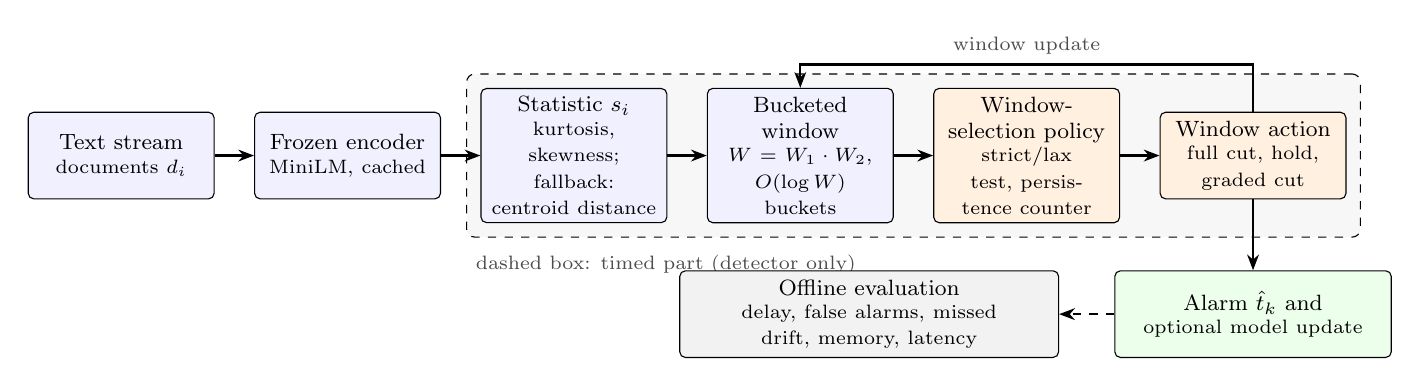
\begin{tikzpicture}[
  box/.style={draw, rounded corners=2pt, align=center, minimum height=11mm, text width=2.15cm, inner sep=3pt, font=\footnotesize, fill=blue!6},
  arr/.style={-{Stealth[length=2mm]}, thick},
  lab/.style={font=\scriptsize, text=black!70}
]
\node[box] (n1) {Text stream\\[-1pt]{\scriptsize documents $d_i$}};
\node[box, right=5mm of n1] (n2) {Frozen encoder\\[-1pt]{\scriptsize MiniLM, cached}};
\node[box, right=5mm of n2] (n3) {Statistic $s_i$\\[-1pt]{\scriptsize kurtosis, skewness; fallback: centroid distance}};
\node[box, right=5mm of n3] (n4) {Bucketed window\\[-1pt]{\scriptsize $W=W_1\cdot W_2$, $O(\log W)$ buckets}};
\node[box, right=5mm of n4, fill=orange!12] (n5) {Window-selection policy\\[-1pt]{\scriptsize strict/lax test, persistence counter}};
\node[box, right=5mm of n5, fill=orange!12] (n6) {Window action\\[-1pt]{\scriptsize full cut, hold, graded cut}};
\foreach \a/\b in {n1/n2,n2/n3,n3/n4,n4/n5,n5/n6}{\draw[arr] (\a) -- (\b);}
\draw[arr] (n6.north) -- ++(0,6mm) -| node[lab, pos=0.25, above] {window update} (n4.north);
\begin{scope}[on background layer]
\node[draw, dashed, rounded corners=3pt, inner sep=5pt, fit=(n3)(n4)(n5)(n6), fill=black!3] (timed) {};
\end{scope}
\node[lab, anchor=north west] at ([yshift=-1mm]timed.south west) {dashed box: timed part (detector only)};
\node[box, below=9mm of n6, text width=3.3cm, fill=green!8] (out) {Alarm $\hat t_k$ and\\[-1pt]{\scriptsize optional model update}};
\node[box, left=7mm of out, text width=4.6cm, fill=gray!10] (ev) {Offline evaluation\\[-1pt]{\scriptsize delay, false alarms, missed drift, memory, latency}};
\draw[arr] (n6.south) -- (out.north);
\draw[arr, dashed] (out.west) -- (ev.east);
\end{tikzpicture}
\caption{Overview of the proposed pipeline. Embeddings are computed once and cached, so the timed part covers only the detector. The orange boxes mark the new component.}
\label{fig:pipeline}
\end{figure*}

\subsection{Problem setting}

The stream is a sequence of documents $d_1,d_2,\dots$ arriving one at a time. Each document is mapped to an embedding $x_i$ by a frozen encoder. The detector sees only $x_i$, never a label, and outputs alarm times. Labels are used only to build streams with known drift and to train an optional downstream classifier. The goal is to alarm soon after each true drift, raise few alarms when nothing changed, miss no drift, and stay within streaming time and memory limits.

\subsection{Pipeline overview}

Fig.~\ref{fig:pipeline} shows the pipeline. Documents are encoded once with a frozen Sentence-BERT model (\texttt{all-MiniLM-L6-v2}, distilled from MiniLM \cite{wang2020}), and the vectors are cached, so detector timings exclude encoding. Following ADWIN-U, the detector computes one scalar statistic $s_i$ per embedding, such as kurtosis or skewness over its components, and inserts it into ADWIN's bucketed window. Since topic drift may not change these statistics, we test this first and keep the cosine distance to the window centroid as a fallback. After each check, the policy looks at the evidence and applies one window action.



\subsection{Window-selection policy}

The window $W$ is split into an older part $W_1$ and a recent part $W_2$, and the signed gap of their means is $g=\hat\mu_{W_1}-\hat\mu_{W_2}$. ADWIN-U cuts $W_1$ when $|g|$ exceeds one bound $\varepsilon$ derived from a Hoeffding-type inequality \cite{bifet2007}. Our policy computes the bound at a strict level $\delta_s$ and a lax level $\delta_w>\delta_s$, giving $\varepsilon_s>\varepsilon_w$, and adds a persistence counter $c$. Fig.~\ref{fig:states} shows the logic. A strong gap ($|g|\ge\varepsilon_s$) causes a full cut, as in ADWIN-U. A weak gap ($\varepsilon_w\le|g|<\varepsilon_s$) starts a hold: the window is not cut, a warning is raised, and $c$ counts consecutive weak checks with the same sign of $g$. If the gap vanishes or changes sign, the hold is released. If it persists for $k$ checks, a graded cut is applied.

\begin{figure}[!t]
\centering
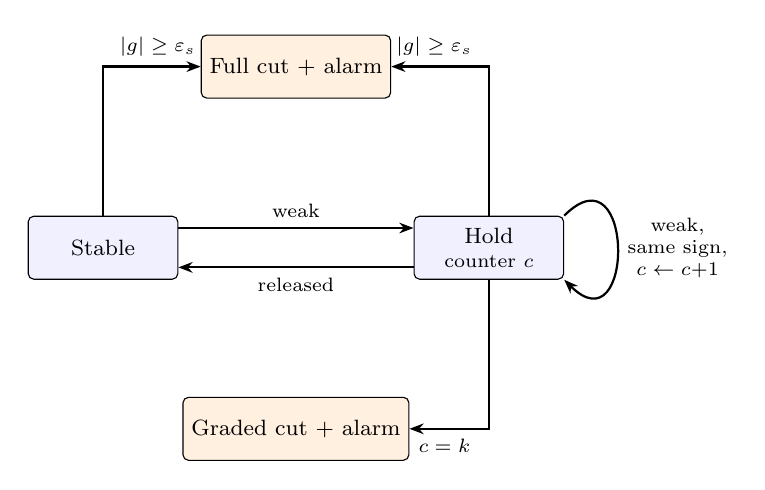
\begin{tikzpicture}[
  st/.style={draw, rounded corners=2pt, align=center, minimum height=8mm, minimum width=1.9cm, inner sep=3pt, font=\footnotesize, fill=blue!6},
  ac/.style={draw, rounded corners=2pt, align=center, minimum height=8mm, inner sep=3pt, font=\footnotesize, fill=orange!12},
  arr/.style={-{Stealth[length=1.8mm]}, thick},
  lab/.style={font=\scriptsize, align=center}
]
\node[st] (stable) at (0,0) {Stable};
\node[st] (hold) at (4.9,0) {Hold\\[-1pt]{\scriptsize counter $c$}};
\node[ac] (full) at (2.45,2.3) {Full cut + alarm};
\node[ac] (grad) at (2.45,-2.3) {Graded cut + alarm};
\draw[arr] (stable.north) |- node[lab, pos=0.78, above] {$|g|\ge\varepsilon_s$} (full.west);
\draw[arr] (hold.north) |- node[lab, pos=0.78, above] {$|g|\ge\varepsilon_s$} (full.east);
\draw[arr] ([yshift=2.5mm]stable.east) -- node[lab, above] {weak} ([yshift=2.5mm]hold.west);
\draw[arr] ([yshift=-2.5mm]hold.west) -- node[lab, below] {released} ([yshift=-2.5mm]stable.east);
\draw[arr] (hold.south) |- node[lab, pos=0.78, below] {$c=k$} (grad.east);
\draw[arr] (hold.north east) .. controls +(0.9,0.9) and +(0.9,-0.9) .. node[lab, right, pos=0.5] {weak,\\same sign,\\$c\leftarrow c{+}1$} (hold.south east);
\end{tikzpicture}
\caption{States of the window-selection policy. A strong gap always triggers a full cut. A weak gap starts a hold, which ends in a graded cut after $k$ consistent checks, or is released when the gap vanishes or changes sign. After either cut the policy returns to Stable.}
\label{fig:states}
\end{figure}

The graded cut drops only the oldest share $\rho=\min(1,|g|/\varepsilon_s)$ of $W_1$, so a larger gap removes more (Fig.~\ref{fig:cuts}). The reason to expect a gain is that a gradual or subtle drift may keep $|g|$ below $\varepsilon_s$ for a long time, even though the old data already differ from the new data. A persistent weak gap is evidence of this, and the hold state keeps a one-off blip from causing a cut.

\begin{figure}[!t]
\centering
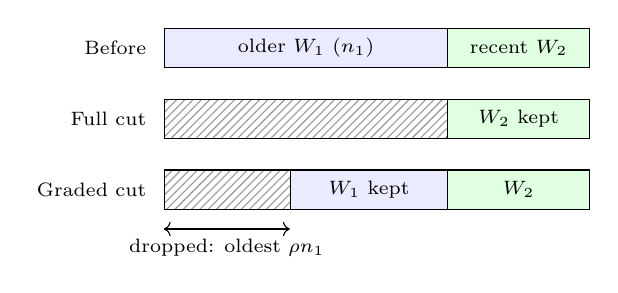
\begin{tikzpicture}[
  seg/.style={draw, minimum height=5mm, inner sep=0pt, font=\scriptsize},
  lab/.style={font=\scriptsize, anchor=east}
]
\def\a{3.6} \def\b{1.8} \def\d{1.6} \pgfmathsetmacro{\r}{\a-\d}
\node[lab] at (0,0) {Before};
\node[seg, minimum width=\a cm, fill=blue!8, anchor=west] (a1) at (0.1,0) {older $W_1$ ($n_1$)};
\node[seg, minimum width=\b cm, fill=green!12, anchor=west] (a2) at (\a+0.1,0) {recent $W_2$};
\node[lab] at (0,-0.9) {Full cut};
\node[seg, minimum width=\a cm, pattern=north east lines, pattern color=black!40, anchor=west] at (0.1,-0.9) {};
\node[seg, minimum width=\b cm, fill=green!12, anchor=west] at (\a+0.1,-0.9) {$W_2$ kept};
\node[lab] at (0,-1.8) {Graded cut};
\node[seg, minimum width=\d cm, pattern=north east lines, pattern color=black!40, anchor=west] at (0.1,-1.8) {};
\node[seg, minimum width=\r cm, fill=blue!8, anchor=west] at (\d+0.1,-1.8) {$W_1$ kept};
\node[seg, minimum width=\b cm, fill=green!12, anchor=west] at (\a+0.1,-1.8) {$W_2$};
\draw[<->, thin] (0.1,-2.3) -- node[font=\scriptsize, below] {dropped: oldest $\rho n_1$} (\d+0.1,-2.3);
\end{tikzpicture}
\caption{Window after a full cut (all of $W_1$ dropped, hatched) and after a graded cut (only the oldest part of $W_1$ dropped).}
\label{fig:cuts}
\end{figure}

Three design points complete the picture. If $\delta_w=\delta_s$ the weak zone is empty and the policy equals ADWIN-U, so ADWIN-U is a special case. The policy adds only a counter and a sign per check and cuts whole buckets, so we expect ADWIN-U's $O(\log W)$ cost to remain, which we will measure. The lax test does not carry the strict bound's false-alarm guarantee once persistence is used, so we will measure false alarms on drift-free streams. The parameters $\delta_s$, $\delta_w$, $k$, and $\rho$ are open choices to tune and ablate.

\subsection{Evaluation plan}

\paragraph{Data}
We build drift on AG News \cite{zhang2015} by changing the topic mix: a switch at one point for abrupt drift, a sigmoid transition for gradual drift \cite{bifet2010}, and a return to an earlier mix for recurring drift. On 20 Newsgroups \cite{lang1995}, swapping groups from different macro-topics gives strong drift, and swapping sibling groups gives subtle drift. As a real stream we use timestamped Amazon reviews \cite{ni2019} in time order. Its drift points are unknown, so we use proxies: alarm rate, downstream accuracy for a given label budget, and alignment with a known event.

\paragraph{Baselines and metrics}
We compare against ADWIN-U (single and multiple detectors), plain ADWIN with a grid of $\delta$ values, a two-threshold warning/alarm variant, a KSWIN-style fixed-window test \cite{raab2020}, and a D3-style discriminative detector \cite{gozuacik2019}. The first three address the objection that any gain comes only from tuning $\delta$ or adding a warning zone. We report mean time to detection, false alarms per 1,000 instances, missed-drift rate, window length, per-instance latency, and peak memory, with BAR \cite{assis2025} as a secondary score. Detectors are first set to the same false-alarm rate on a drift-free stream, run on several random stream orders, and ranked with the Friedman and Nemenyi tests \cite{demsar2006}. Ablations (hold only, graded cut without persistence, full policy) show which part matters.

\paragraph{Hypotheses}
At the same false-alarm rate, we expect lower delay than ADWIN-U on gradual and subtle drift, similar results on abrupt strong drift, and a small constant extra cost per instance. Each can turn out false.

%--------------------------------------------------------------------
\section{Current Status and Next Steps}
\label{sec:status}

So far we have completed the literature review, defined the policy and its parameters, and fixed the datasets and evaluation protocol. No experimental results exist yet, and none are reported here. The next steps are:
(1) reproduce ADWIN-U on text embeddings, using the authors' released code as a starting point, and check whether kurtosis and skewness respond to topic drift, with centroid distance as the fallback;
(2) implement the policy on the bucketed window and verify that $\delta_w=\delta_s$ gives the same alarms as ADWIN-U;
(3) generate the injected-drift streams and run the baselines and ablations;
(4) run the real review stream with the proxy measures; and
(5) finish the systematic literature search to confirm what is new.

The main risk is step (1). If the per-example statistics do not react to topic change, the detector will have nothing to act on, and the policy will have to use a different monitored value. We consider this a finding worth reporting in either case.

%--------------------------------------------------------------------
\begin{thebibliography}{99}
\bibitem{gama2014} J.~Gama, I.~\v{Z}liobait\.{e}, A.~Bifet, M.~Pechenizkiy, and A.~Bouchachia, ``A survey on concept drift adaptation,'' \emph{ACM Comput.\ Surv.}, vol.~46, no.~4, art.~44, 2014.

\bibitem{lu2019} J.~Lu, A.~Liu, F.~Dong, F.~Gu, J.~Gama, and G.~Zhang, ``Learning under concept drift: A review,'' \emph{IEEE Trans.\ Knowl.\ Data Eng.}, vol.~31, no.~12, pp.~2346--2363, 2019.

\bibitem{garcia2024review} C.~M. Garcia, R.~S. Abilio, A.~L. Koerich, A.~S. Britto~Jr., and J.~P. Barddal, ``Concept drift adaptation in text stream mining settings: A systematic review,'' \emph{ACM Trans.\ Intell.\ Syst.\ Technol.}, 2024, doi:10.1145/3704922.

\bibitem{hinder2024a} F.~Hinder, V.~Vaquet, and B.~Hammer, ``One or two things we know about concept drift---a survey on monitoring in evolving environments. Part A: Detecting concept drift,'' \emph{Front.\ Artif.\ Intell.}, vol.~7, 2024, doi:10.3389/frai.2024.1330257.

\bibitem{lukats2025} D.~Lukats, O.~Zielinski, A.~Hahn, and F.~Stahl, ``A benchmark and survey of fully unsupervised concept drift detectors on real-world data streams,'' \emph{Int.\ J.\ Data Sci.\ Anal.}, vol.~19, pp.~1--31, 2025.

\bibitem{bifet2007} A.~Bifet and R.~Gavald\`a, ``Learning from time-changing data with adaptive windowing,'' in \emph{Proc.\ SIAM Int.\ Conf.\ Data Mining}, 2007, pp.~443--448.

\bibitem{assis2025} D.~N. Assis and V.~M.~A. Souza, ``ADWIN-U: Adaptive windowing for unsupervised drift detection on data streams,'' \emph{Knowl.\ Inf.\ Syst.}, vol.~67, no.~11, pp.~10005--10034, 2025.

\bibitem{webb2016} G.~I. Webb, R.~Hyde, H.~Cao, H.~L. Nguyen, and F.~Petitjean, ``Characterizing concept drift,'' \emph{Data Min.\ Knowl.\ Discov.}, vol.~30, no.~4, pp.~964--994, 2016.

\bibitem{suarez2023} A.~L. Su\'arez-Cetrulo, D.~Quintana, and A.~Cervantes, ``A survey on machine learning for recurring concept drifting data streams,'' \emph{Expert Syst.\ Appl.}, vol.~213, art.~118934, 2023.

\bibitem{gama2004} J.~Gama, P.~Medas, G.~Castillo, and P.~Rodrigues, ``Learning with drift detection,'' in \emph{Advances in Artificial Intelligence (SBIA)}, LNAI vol.~3171, 2004, pp.~286--295.

\bibitem{raab2020} C.~Raab, M.~Heusinger, and F.-M. Schleif, ``Reactive soft prototype computing for concept drift streams,'' \emph{Neurocomputing}, vol.~416, pp.~340--351, 2020.

\bibitem{gozuacik2019} \"O.~G\"oz\"u\c{c}\i k, A.~Bifet, and F.~Can, ``Unsupervised concept drift detection with a discriminative classifier,'' in \emph{Proc.\ ACM Int.\ Conf.\ Inf.\ Knowl.\ Manag. (CIKM)}, 2019, pp.~2365--2368.

\bibitem{hoeffding1963} W.~Hoeffding, ``Probability inequalities for sums of bounded random variables,'' \emph{J.\ Amer.\ Statist.\ Assoc.}, vol.~58, no.~301, pp.~13--30, 1963.

\bibitem{datar2002} M.~Datar, A.~Gionis, P.~Indyk, and R.~Motwani, ``Maintaining stream statistics over sliding windows,'' \emph{SIAM J.\ Comput.}, vol.~31, no.~6, pp.~1794--1813, 2002.

\bibitem{hinder2020} F.~Hinder, A.~Artelt, and B.~Hammer, ``Towards non-parametric drift detection via dynamic adapting window independence drift detection (DAWIDD),'' in \emph{Proc.\ Int.\ Conf.\ Mach.\ Learn.\ (ICML)}, PMLR vol.~119, 2020, pp.~4249--4259.

\bibitem{chen2024} J.~Chen, S.~Yang, T.~Gao, Y.~Ying, T.~Li, and P.~Li, ``Multi-type concept drift detection under a dual-layer variable sliding window in frequent pattern mining with cloud computing,'' \emph{J.\ Cloud Comput.}, vol.~13, art.~40, 2024.

\bibitem{klinkenberg2000} R.~Klinkenberg and T.~Joachims, ``Detecting concept drift with support vector machines,'' in \emph{Proc.\ Int.\ Conf.\ Mach.\ Learn.\ (ICML)}, 2000, pp.~487--494.

\bibitem{kuncheva2009} L.~I. Kuncheva and I.~\v{Z}liobait\.{e}, ``On the window size for classification in changing environments,'' \emph{Intell.\ Data Anal.}, vol.~13, no.~6, pp.~861--872, 2009.

\bibitem{mehmood2024} H.~Mehmood, A.~Khalid, P.~Kostakos, E.~Gilman, and S.~Pirttikangas, ``A novel edge architecture and solution for detecting concept drift in smart environments,'' \emph{Future Gener.\ Comput.\ Syst.}, vol.~150, pp.~127--143, 2024.

\bibitem{badar2023} M.~Badar, W.~Nejdl, and M.~Fisichella, ``FAC-fed: Federated adaptation for fairness and concept drift aware stream classification,'' \emph{Mach.\ Learn.}, vol.~112, pp.~2761--2786, 2023.

\bibitem{hu2024} L.~Hu, W.~Li, Y.~Lu, and C.~Hu, ``Scalable concept drift adaptation for stream data mining,'' \emph{Complex Intell.\ Syst.}, vol.~10, pp.~6725--6743, 2024.

\bibitem{reimers2019} N.~Reimers and I.~Gurevych, ``Sentence-BERT: Sentence embeddings using Siamese BERT-networks,'' in \emph{Proc.\ EMNLP-IJCNLP}, 2019, pp.~3982--3992.

\bibitem{wang2020} W.~Wang, F.~Wei, L.~Dong, H.~Bao, N.~Yang, and M.~Zhou, ``MiniLM: Deep self-attention distillation for task-agnostic compression of pre-trained transformers,'' in \emph{Advances in Neural Information Processing Systems}, vol.~33, 2020, pp.~5776--5788.

\bibitem{zhang2015} X.~Zhang, J.~Zhao, and Y.~LeCun, ``Character-level convolutional networks for text classification,'' in \emph{Advances in Neural Information Processing Systems}, vol.~28, 2015.

\bibitem{lang1995} K.~Lang, ``NewsWeeder: Learning to filter netnews,'' in \emph{Proc.\ Int.\ Conf.\ Mach.\ Learn.\ (ICML)}, 1995, pp.~331--339.

\bibitem{ni2019} J.~Ni, J.~Li, and J.~McAuley, ``Justifying recommendations using distantly-labeled reviews and fine-grained aspects,'' in \emph{Proc.\ EMNLP-IJCNLP}, 2019, pp.~188--197.

\bibitem{bifet2010} A.~Bifet, G.~Holmes, R.~Kirkby, and B.~Pfahringer, ``MOA: Massive online analysis,'' \emph{J.\ Mach.\ Learn.\ Res.}, vol.~11, pp.~1601--1604, 2010.

\bibitem{demsar2006} J.~Dem\v{s}ar, ``Statistical comparisons of classifiers over multiple data sets,'' \emph{J.\ Mach.\ Learn.\ Res.}, vol.~7, pp.~1--30, 2006.
\end{thebibliography}

\end{document}
